\section{B-splines - basic splines}
\begin{frame}
	$B_{j,k}(x)$ - B-spline rzędu k:
    \begin{itemize}
    \item  $B_{j,1}=
        \begin{cases}
            	1  &,\ x_{j} \leq x \leq x_{j+1}
            	\\
                0 &,\ \textrm{poza przedziałem}
        \end{cases}
        $
        \item wyższe rzędy $(k>1)$ - rekurencyjnie:
        \[
        	B_{j,k}=\frac{x-x_{j}}{x_{j+k-1}-x_{j}}B_{j,k-1}(x)+\frac{x_{j+k}-x}
            {x_{j+k}-x_{j+1}}B_{j+1,k-1}(x)
        \]
        \item $B_{j,k}(x)=\{>0, x\in[x_{j},\ x_{j+k}]=0\} \ \ x 
        \textrm{- poza przedziałem}$
        \item w przedziale $[x_{j},\ x_{j+1}]$ tylko $k$: $B_{j-k+1,k}(x)\ldots
        B_{j,k}(x)\neq 0$
		\item normalizacja: $\sum_{j}B_{j,k}(x)=\sum_{j=l+1-k}^{l}B_{j,k}(x)=1$ 
        \newline dla $x_{l}\leq x\leq x_{l+1}$
\end{itemize}
\end{frame}
%%%%%%%%%%%%%%%%%%%%%%%%
\begin{frame}
	\begin{exampleblock}{Reprezentacja funkcji sklejanej stopnia k-1}
		\centering $S(x)=\sum_{j}a_{j}B_{j,k}(x)$
	\end{exampleblock}
    $k=4 \rightarrow$ cubic B-splines: $B_{j,4}(x)=b_{j}(x)$
    $
    \begin{rcases*}
			x \in [a,b]\\
			m - \textrm{B-splines} \ \  b_{j}(x)
		\end{rcases*}\Rightarrow \textrm{odległość między sąsiednimi węzłami}
    $
    $\newline \newline \newline$
    $d = \frac{b-a}{m-3} \newline$
    $(m+4) \textrm{węzły} \ \newline$
    $x_{4}=a \newline$
    $x_{m+1}=b \newline$
    $x_{j}=a+(j-4)d$
\end{frame}
%%%%%%%%%%%%%%%%%%%%%%%%
\begin{frame}
	\begin{figure}[h]
			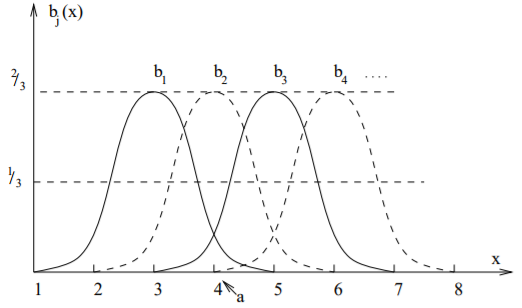
\includegraphics[width=.57\linewidth]{img/4/spline_img_6}
	\end{figure}
    \begin{block}{Zadanie}
    	$B_{j,k}$ dla równoodległych węzłów
    \end{block}
    \[	b_{j}(x)=
    	\begin{cases}
    		\frac{1}{6}z^{3} &,z=\frac{x-x_{j}}{d} \ \ x \in [x_{j},x_{j+1}] \\
            \frac{1}{6}[1+3(1+z(1-z))z] &,z=\frac{x-x_{j+1}}{d} \ x 
            \in [x_{j+1},x_{j+2}]\\
            \frac{1}{6}[1+3(1+z(1-z))(1-z)] &,z=\frac{x-x_{j+2}}{d} \ x 
            \in [x_{j+2},x_{j+3}] \\
            \frac{1}{6}(1-z)^{3} &,z=\frac{x-x_{j+3}}{d} \ x 
            \in [x_{j+3},x_{j+4}] \\
            0 \ &, x \notin [x_{j},x_{j+4}]
    	\end{cases}
    \]
\end{frame}
%%%%%%%%%%%%%%%%%%%%%%%%
\begin{frame}{Zastosowanie}
	\begin{itemize}
	\item ogólne zastosowanie B-spline'ów - 
    	$\newline$encyklopedia matematyczna $\newline$
    		(autor: Copenhagen University Astronomical Observatory)
    \item w grafice komputerowej %deadlink
	\end{itemize}
\end{frame}
%%%%%%%%%%%%%%%%%%%%%%%
\begin{frame}
	\begin{figure}[h]
			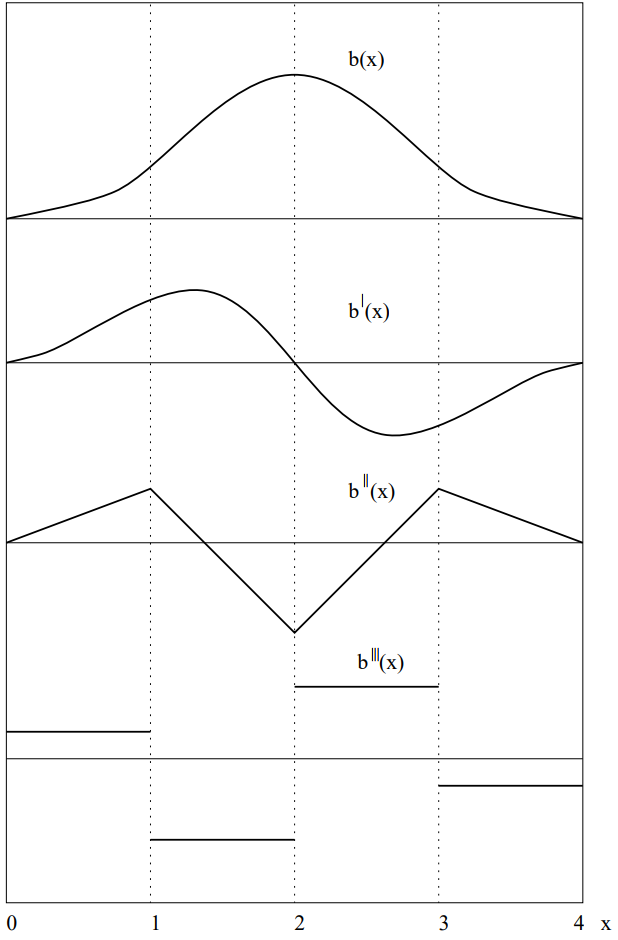
\includegraphics[width=.52\linewidth]{img/4/spline_img_7}
	\end{figure}
\end{frame}




